\documentclass{sigplanconf}

\usepackage{caption}
\DeclareCaptionType{copyrightbox}

\usepackage{amsmath,amsthm,amssymb,stmaryrd}
\usepackage{graphicx}
\usepackage{epstopdf}
\usepackage{MnSymbol}
\usepackage{paralist}
\usepackage{epsfig}
\usepackage{wrapfig}
\usepackage{color}
\usepackage{program}
\usepackage{multirow}
\usepackage{rotating}
\usepackage{subfig} 
\usepackage{proof}
\usepackage{hyperref}
%\usepackage[normalem]{ulem}


\usepackage{supertabular}

\newcommand\TRUE{\textsf{true}}
\newcommand\FALSE{\textsf{false}}

\newcommand\APP{{\sc app}}
\newcommand\UNAPP{{\sc unapp}}
\newcommand\PUSH{{\sc push}}
\newcommand\UNPUSH{{\sc unpush}}
\newcommand\PULL{{\sc pull}}
\newcommand\UNPULL{{\sc unpull}}
\newcommand\CMT{{\sc cmt}}

\newcommand\gCommitted{\textsf{gCmt}}
\newcommand\gUncommitted{\textsf{gUCmt}}

\newcommand\lPushed{\small\textsf{pushed}}
\newcommand\lUnpushed{\small\textsf{unpushed}}
\newcommand\lPulled{\small\textsf{pulled}}
\newcommand\lCommitted{\small\textsf{cmted}}

\newcommand\x{\texttt{x}}
\newcommand\y{\texttt{y}}

%\newcommand\pmpyreduce{\leadsto}
\newcommand\pmpyreduce{\xrightarrow{\;\;\;}}
\newcommand\pmpyrt{\xrightarrow{\textsf{rt}}}
\newcommand\pmpyfwd{\xrightarrow{\textsf{fwd}}}
\newcommand\pmpyback{\xrightarrow{\textsf{back}}}
\newcommand\pmpystruct{\xrightarrow{\textsf{struct}}}

%%% Local Variables: 
%%% mode: plain-tex
%%% TeX-master: "paper"
%%% End: 

\newcommand\tx[1]{\texttt{tx}\ #1}
\newcommand\skipt{\texttt{skip}}
\newcommand\plust{\texttt{ + }}
\newcommand\semit{\texttt{ ; }}
\newcommand\opname{m}
\newcommand\op{op}
\newcommand\step[1]{\textsf{step}(#1)}
\newcommand\nothingtext{fin}
\newcommand\nothing[1]{\textsf{\nothingtext}(#1)}
\newcommand\committ{\textsf{cmt}}
\newcommand\lstack{\sigma}
\newcommand\opid{\mathit{id}}
\newcommand\fresh[1]{\textsf{fresh}(#1)}
\newcommand\OPL{\ell} 
\newcommand\unpushed[1]{\lfloor #1 \rfloor_{\lUnpushed}}
\newcommand\pushed[1]{\lfloor #1 \rfloor_{\lPushed}}
\newcommand\pulled[1]{\lfloor #1 \rfloor_{\lPulled}}
\newcommand\gcommitted[1]{\lfloor #1 \rfloor_{\gCommitted}}
\newcommand\guncommitted[1]{\lfloor #1 \rfloor_{\gUncommitted}}
\newcommand\MOR{\;\mid\;}
\newcommand\allowedt{\textsf{allowed}}
\newcommand\allowed[1]{\allowedt\ #1}
\newcommand\allows{\textsf{ allows }}
\newcommand\opeq{\preccurlyeq} %\asymp}
% \newcommand{\ottdefnaMachHACK}[1]{\begin{ottdefnblock}[#1]{$\ottnt{c_{{\mathrm{1}}}}  \ottsym{,}  \sigma_{{\mathrm{1}}}  \ottsym{,}  \OPL  \xrightarrow{a}  \ottnt{c_{{\mathrm{2}}}}  \ottsym{,}  \sigma_{{\mathrm{2}}}  \ottsym{,}  \OPL$}{}
\newcommand\As{\mathbf{A}}
\newcommand\Ts{\mathbf{T}}
% \newcommand{\ottdefngMachStarHACK}[1]{\begin{ottdefnblock}[#1]{$\mathbf{T}_{{\mathrm{1}}}  \ottsym{,}  \ottnt{G_{{\mathrm{1}}}}  \pmpyreduce^{*}  \mathbf{T}_{{\mathrm{2}}}  \ottsym{,}  \ottnt{G_{{\mathrm{2}}}}$}{}
\newcommand\lm[2]{#1 \ \blacktriangleleft\ #2}



\newcommand\SimRel{\;\sim\;}
%\newcommand\theOP{\langle m, \sigma, \vec{a}, \sigma', \vec{r}, \opid \rangle}
%\newcommand\numOP[1]{\langle m_#1, \sigma_#1, \vec{a}_#1, \sigma'_#1, \vec{r}_#1, \opid_#1\rangle}
\newcommand\theOP{\langle m, \sigma, \sigma', \opid \rangle}
\newcommand\numOP[1]{\langle m_#1, \sigma_#1, \sigma'_#1, \opid_#1\rangle}
\newcommand\cmtpres{\textsf{cmtpres}}
\newcommand\prewind{\;\circlearrowleft\;}
\newcommand\Gpost{G_\textsf{post}}
\newcommand\numCSL[1]{\{c_{#1}, \sigma_{#1}, L_{#1}\}}
\newcommand\CSL{\{c, \sigma, L\}}
\newcommand\CpSpLp{\{c', \sigma', L'\}}
\newcommand\CSLp{\{c, \sigma, L'\}}
\newcommand\csL[1]{\{c, \sigma, #1\}}
\newcommand\cslCS[2]{\{#1, #2, L\}}
\newcommand\cslCSL[3]{\{#1, #2, #3\}}
\newcommand\cslpre{\{`c, `\sigma, `L\}}
\newcommand\Gothers{G\setminus \pushed{L_1\cdot\hat{L}_2}}
\newcommand\Gmine{G\cap \pushed{L_1\cdot\hat{L}_2}}
\newcommand\invA{\textsf{inv}_a}
\newcommand\invAC{\textsf{inv}_{ac}}
\newcommand\invB{\textsf{inv}_b}
\newcommand\invBC{\textsf{inv}_{bc}}
\newcommand\early[3]{\textsf{early }#1\textsf{ then }#2\textsf{ in }#3}
\newcommand\invC{\textsf{inv}_c}
\newcommand\invCC{\textsf{inv}_{cc}}
% \newcommand\invBC{\textsf{inv}_{bc}}
% \newcommand\invar[4]{\begin{array}{ll}%
% \newcommand\invarCSLG{\invar{c}{\sigma}{L}{G}}

%%% Local Variables: 
%%% mode: plain-tex
%%% TeX-master: "paper"
%%% End: 


% program listings
\usepackage{listings}
\lstset{language=java,columns=flexible,numberstyle=\tiny,showstringspaces=false,basicstyle=\sffamily} %,frame=single
\lstset{escapechar=`}
\lstset{morekeywords={
        var, val}}

\newcommand{\juc}{\lstinline+java+.\!\lstinline+util+.\lstinline+concurrent+}
\newcommand{\cConcurrentSkipListMap}{\lstinline+ConcurrentSkipListMap+}

\newtheorem{theorem}{Theorem}[section]
\newtheorem{lemma}[theorem]{Lemma}
\newtheorem{proposition}[theorem]{Proposition}
\newtheorem{corollary}[theorem]{Corollary}
\newtheorem{definition}{Definition}[section]
\newtheorem{parameter}{Parameter}[section]
\newtheorem{property}{Property}[section]
\newtheorem{example}[equation]{Example}
\newtheorem{algorithm}[theorem]{Algorithm}

\newenvironment{itemize*}%
  {\begin{itemize}%
    \setlength{\itemsep}{0.0in}%
    \setlength{\topsep}{0.0in}%
    \setlength{\parskip}{0.0in}}%
  {\end{itemize}}
\newenvironment{enumerate*}%
  {\begin{enumerate}%
    \setlength{\itemsep}{0.0in}%
    \setlength{\topsep}{0.0in}%
    \setlength{\parskip}{0.0in}}%
  {\end{enumerate}}

% URL macro allows linebreaks on slash
\makeatletter
{\catcode`\/\active\catcode`\_\active\catcode`\.\active
\gdef\URLslash{\futurelet\next\@@URLslash}%
\gdef\@@URLslash{\ifx\next\URLslash\char`\/\else\slash\fi}%
\gdef\URLdot{\char`\.\penalty\exhyphenpenalty}%
\gdef\URLprepare{\catcode`\/\active\catcode`\_\active\catcode`\.\active
        \let/\URLslash\let.\URLdot\def~{\char`\~}\def_{\char`\_}}}%
\def\URL{\bgroup\URLprepare\realURL}%
\def\realURL#1{\tt #1\egroup}%




\definecolor{light-gray}{gray}{0.85}
\newcommand\todo[1]{{\color{red} \textbf{#1}}}
%\newcommand\todo[1]{[[[#1]]]}
\newcommand\esays[1]{\todo[color=blue!40]{{\bf E says:} #1}}
\newcommand\msays[1]{\todo[color=red!40]{{\bf M says:} #1}}
\newcommand\whitetext[1]{{\color{white} #1}}
\newcommand\red[1]{{\color{red} #1}}
\newcommand\blue[1]{{\color{blue} #1}}
\newcommand\comment[1]{{\color{blue} #1}}
\newcommand\ignore[1]{}
\newcommand\disabled[1]{{\color{light-gray} #1}}
\newcommand\eg{{\it e.g.}}
\newcommand\ie{{\it i.e.}}
\newcommand\cf{{\it cf.}}

\newcommand\FULL[1]{}
\newcommand\SHORT[1]{#1}
\newcommand\BLIND[1]{}
\newcommand\NOTBLIND[1]{#1}

\newcommand\figbox[1]{\noindent{\ \\\fbox{\begin{minipage}{3.2in}
#1
\end{minipage}
}}}

\newcommand\figboxB[1]{\noindent{\ \\\fbox{\begin{minipage}{6.5in}
#1
\end{minipage}
}}}

\newcommand{\labels}{\ensuremath{\mathsf{Lab}}}
\newcommand{\edges}{\ensuremath{\mathsf{Edg}}}
\newcommand{\actions}{\ensuremath{\mathsf{Act}}}
\newcommand{\cfg}{\ensuremath{\mathsf{CFG}}}
\newcommand{\getaction}[2]{\ensuremath{\cfunction{getAct(#1, #2)}}}
\newcommand{\replace}[3]{\ensuremath{\cfunction{rep}(#1, #2, #3)}}
\newcommand{\extractstep}[3]{\ensuremath{\cfunction{extractStep}(#1, #2, #3)}}

\newcommand{\naturalnumbers}{\ensuremath{\mathbb{N}}}

\newcommand{\parts}[1]{\ensuremath{\wp(#1)}}
\newcommand{\dom}[1]{\ensuremath{\cfunction{dom}(#1)}}
\newcommand{\statement}[1]{\ensuremath{\mathtt{#1}}}
\newcommand{\funzione}[2]{\ensuremath{#1 \rightarrow#2}}
\newcommand{\trace}[1]{\ensuremath{#1^{\vec{+}}}}
\newcommand{\pair}[2]{\ensuremath{#1 \times #2}}
\newcommand{\triple}[3]{\ensuremath{#1 \times #2 \times #3}}
\newcommand{\cartesianproduct}[2]{\ensuremath{#1 \times #2}}
\newcommand{\reducedproduct}[2]{\ensuremath{#1 \varotimes #2}}
\newcommand{\true}{\cel{true}}
\newcommand{\false}{\cel{false}}
\newcommand{\reducefunction}{\afunction{red}}
\newcommand{\sem}[1]{\ensuremath{\llbracket #1 \rrbracket}}
\newcommand{\semanticanome}[1]{\ensuremath{\mathbb{#1}}}
\newcommand{\semantica}[2]{\ensuremath{\semanticanome{#1}\sem{#2}}}
\newcommand{\bigdivision}[2]{\frac{\displaystyle #1}{\displaystyle #2}}

\newcommand{\statements}{\cset{St}}
\newcommand{\states}{\Sigma}
\newcommand{\badtraces}{\cset{BadTraces}}
\newcommand{\goodtraces}{\cset{GoodTraces}}
\newcommand{\nextStatement}[2]{\ensuremath{\cfunction{nextSt}(#1, #2)}}
\newcommand{\lastLabel}[2]{\ensuremath{\cfunction{lastLab}(#1, #2)}}
\newcommand{\projectTrace}[1]{\ensuremath{\pi_\labels(#1)}}
\newcommand{\isBad}[1]{\ensuremath{\cfunction{isBad}(#1)}}
\newcommand{\getTransactionPoints}[1]{\ensuremath{\cfunction{transPP}(#1)}}
\newcommand{\indexes}[2]{\ensuremath{\cfunction{indexes}(#1, #2)}}
\newcommand{\observe}[1]{\ensuremath{\cfunction{observe}(#1)}}


%Concreto

%Dominio e semantica concrete
\newcommand{\cset}[1]{\ensuremath{\mathsf{#1}}}
\newcommand{\cstates}{\ensuremath{\cset{\states}}}
\newcommand{\cstatesmemory}{\ensuremath{\cset{\states_m}}}
\newcommand{\ctrace}[1]{\ensuremath{\trace{{\cset{#1}}}}}
\newcommand{\cel}[1]{\ensuremath{\mathsf{#1}}}
\newcommand{\cjoin}{\ensuremath{\cup}}
\newcommand{\cmeet}{\ensuremath{\cap}}
\newcommand{\corder}{\ensuremath{\subseteq}}
\newcommand{\cbot}{\ensuremath{\emptyset}}
\newcommand{\ctop}[1]{\cset{#1}}
\newcommand{\cfunction}[1]{\ensuremath{\mathit{#1}}}
\newcommand{\csemantics}[2]{\ensuremath{\semantica{#1}{#2}}}

%Astratto

%Dominio e semantica astratte
\newcommand{\aset}[1]{\cset{\overline{#1}}}
\newcommand{\astates}{\ensuremath{\aset{\states}}}
\newcommand{\ael}[1]{\cel{\overline{#1}}}
\newcommand{\ajoin}{\ensuremath{\sqcup}}
\newcommand{\ameet}{\ensuremath{\sqcap}}
\newcommand{\awidening}{\ensuremath{\nabla}}
\newcommand{\aorder}{\ensuremath{\sqsubseteq}}
\newcommand{\abot}{\ensuremath{\bot}}
\newcommand{\abtop}{\ensuremath{\top}}
\newcommand{\asemantics}[2]{\semantica{\afunction{\semanticanome{#1}}}{#2}}
\newcommand{\atrace}[1]{\ensuremath{\trace{#1}}}
\newcommand{\afunction}[1]{\ensuremath{\overline{\mathit{#1}}}}
\newcommand{\asemanticsstatementsname}{\ensuremath{\afunction{\semanticanome{\semanticsstatements}}}}
\newcommand{\asemanticsstatements}[1]{\asemantics{\semanticsstatements}{#1}}



\begin{document}

\title{Corrective Synchronization via Trace Warping}
\conferenceinfo{tbd} {tbd}
\copyrightyear{2015}
\copyrightdata{978-1-4503-0490-0/11/01}
\titlebanner{DRAFT---Do not distribute}

\authorinfo{Anonymous} {} {} 
% \authorinfo{Pietro Ferrara} {IBM T.J. Watson Research Center} {pietroferrara@us.ibm.com} 
% \authorinfo{Eric Koskinen} {IBM T.J. Watson Research Center} {ejk@us.ibm.com} 
% \authorinfo{Peng Liu} {Purdue University} {peng74@cs.purdue.edu} 
% \authorinfo{Omer Tripp} {IBM T.J. Watson Research Center} {otripp@us.ibm.com}

%\authorinfo{omitted for double-blind reviewing}{}{}
\maketitle



\section{Introduction}

Concurrency control is a hard problem. While some thread interleavings are admissible (in particular, if they involve disjoint memory accesses), there are certain interleaving scenarios that must be inibited to ensure serializability \cite{XXX}. The goal is to automatically detect --- with high precision and low overhead --- the inadmissible interleavings, and ensure that that do not take effect.  

Toward this end, there are currently two main synchronization paradigms:
\begin{itemize}
	\item \textit{Pessimistic synchronization}: In this approach, illegal interleaving scenarios are avoided conservatively by blocking the execution of one or more of the concurrent threads until the threat of incorrect execution has passed away. Locks, mutexes and semaphores are all examples of how to enforce mutual exclusion, or pessimistic synchronization.
	\item \textit{Optimistic synchronization}: As an alternative to proactive, or pessimistic, synchronization, optimistic synchronization is essentially a reactive approach. The concurrency control system monitors execution, such that when an illegal interleaving scenario arises, it is detected as such and appropriate remediation steps are taken. A notable instance of this paradigm is transactional memory (TM) \cite{XXX}, where the system logs memory accesses by each of the threads, and is able to reverse the effects of a thread and abort/restart it.
\end{itemize}

\paragraph{Motivation} The pessimistic approach is useful if critical sections are short, there is little available concurrency, and the involved memory locations are well known \cite{XXX}. Optimistic synchronization is most effective when there is a high level of available concurrency. An example is graph algorithms, such as Boruvka, over graphs that are sparse and irregular \cite{XXX}.

Beyond these cases, however, there are many other situations of practical interest. As an illustrative example, we refer to the code fragment in Figure \ref{Fi:introMotivating}, extracted from the {\sf dyuproject} project, where a shared {\tt Map} object, (pointed-to by) {\sf \_convertors}, is manipulated by method {\sf getConvertor()}.

\begin{figure}
	\begin{lstlisting}
public Convertor getConvertor(
      Class cls,boolean create,boolean add) {
  Convertor convertor = _convertors.get(cls.getName());
  if(convertor==null && create) {
    convertor = newConvertor(cls,add);
    _convertors.putIfAbsent(cls.getName(), convertor); }
    return convertor; }
	\end{lstlisting}
	\caption{\label{Fi:introMotivating}Method {\sf getConvertor()} from class {\sf StandardConvertorCache} in project {\sf dyuproject}}
\end{figure}

Assume that different threads invoking this method are all attempting to simultaneously obtain the same {\sf Convertor} object, which has not yet been created. Doing so optimistically would lead to multiple rollbacks, and thus poor performance. Mutual exclusion, on the other hand, would block all threads but one until the operation completes, which is far from optimal if {\sf newConvertor()} is an expensive operation.

\paragraph{Our Approach} We propose a novel synchronization paradigm, which is conceptually different from both the pessimistic and the optimistic approaches. In our approach, dubbed \emph{corrective synchronization}, the correctness of multi-threaded execution is enforced after the fact, similarly to optimistic synchronization, though without rollbacks. Instead, the system automatically compensates, if necessary, for the effects of inadmissible interleavings by rewriting the program state as a transaction completes. This is done while accounting for the behavior of concurrent transactions, so as to guarantee serializability.

To illustrate our approach, we revisit the running example. Assume the following execution history:
\begin{center}
	\begin{tabular}{c||c}
		$T_1$ & $T_2$ \\
		\hline
		${\sf \_convertors.get()} / {\sf null}$ &  \\
															  & ${\sf \_convertors.get()} / {\sf null}$ \\
		${\sf if (...)}$ 								   &							\\
															  & ${\sf if (...)}$ \\
		${\sf newConvertor()} / o_1$		& \\
															  & ${\sf newConvertor()} / o_2$ \\
		${\sf \_convertors.putIfAbsent()} / {\sf null}$ &  \\
									& 		${\sf \_convertors.putIfAbsent()} / o_1$ \\
		${\sf return}\ o_1$ & \\
									& ${\sf return}\ o_2$ \\
	\end{tabular}
\end{center}
This history is clearly nonserializable, as in any serializable history $T_1$ and $T_2$ would return the same {\sf Convertor} instance. Correcting this execution involves the application of two actions to the exit state of $T_2$. First, we point the local variable ${\sf convertor}$ to $o_1$, rather than $o_2$. Second, we fix the mapping under $\_convertors$ for key {\sf cls.getName()} in the same way.

Note that the corrective actions above are of a general form, which is not limited to only two threads. For any number of threads, the corrected state would have one privileged thread deciding the return value (i.e., the value of {\sf convertor}) for all threads, which would also be the value linked by the key under {\sf \_convertors}. Also note that the corrective actions are --- relatively speaking --- inexpensive, especially compared to the alternatives of either blocking or aborting/restarting all threads but one.

Two important challenges that we address in this paper w.r.t. the corrective synchronization paradigm are (i) how to compute correct poststates; and (ii) given an incorrect poststate, how to decide which correct poststate to transition to. We govern our discussion of these challenges by a formal framework, based on the push/pull model for transactions \cite{XXX}, with rigorous soundness guarantees. We also provide a clear statement of the limitations of corrective synchronization.

Beyond the formal details, this paper additionally addresses practical challenges, and in particular the question of how to implement corrective synchronization efficiently, such that it incurs low overhead. To this end, we present a solution based on static analysis to derive the correct poststates in relation to a given prestate. We have implemented a version of the analysis for shared {\sf Map} data structures. {\sf Map}s are used to represent the shared state of many Java programs \cite{XXX}, and so this first step toward a comprehensive static analysis for corrective synchronization is already of practical value.

\paragraph{Contributions} This paper makes the following principal contributions:
\begin{enumerate}
	\item \underline{Corrective synchronization:} We present an alternative to both the pessimistic and the optimistic synchronization paradigms, dubbed \emph{corrective synchronization}, whereby serializability is achieved neither via mutual exclusion nor via rollbacks, but through correction of the poststate according to a relational prestate/poststates specification.
	\item \underline{Formal guarantees:} We provide a formal description of corrective synchronization in terms of the push/pull model for transactions. This includes a correctness (or soundness) proof as well as a clear statement of limitations.
	\item \underline{Static analysis:} We have developed a static analysis to derive the prestate/poststates specification for programs that encode the shared state as one or more assoiciative mappings. We describe the analysis in full formal detail.
	\item \underline{Implementation and evaluation}: We have created a protoype implementation of corrective synchronization assuming the shared state is represented as associative mappings. We discuss techniques and optimizations to achieve low overhead. We present experimental evidence in favor of corrective synchronization, where our subjects are derived from real-world Java applications.
\end{enumerate}

\section{Overview}

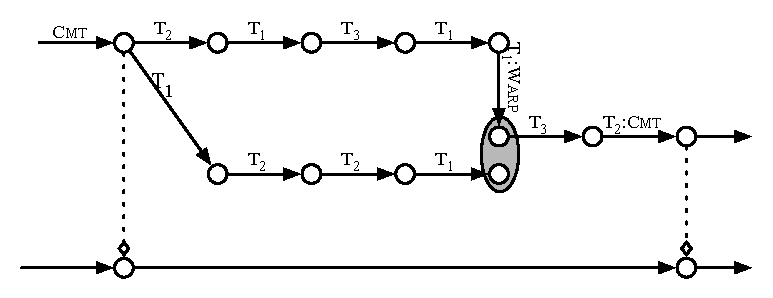
\includegraphics[width=3.2in]{simulation.eps}

\newcommand\obseq{\stackrel{\sim}{=}}
\newcommand\CS{\{c,\sigma\}}
\newcommand\CpSp{\{c',\sigma'\}}
\newcommand\numCS[1]{\{c_{#1},\sigma_{#1}\}}

%\newcommand\cred[3]{#1 \dashrightarrow (#2,#3)}
\newcommand\tstep[3]{#1 \lightning (#2,#3)}
\newcommand\stept{\lightning\!\lightning}
\renewcommand\step[3]{#1 \stept (#2,#3)}

\newcommand\BigStep{\Downarrow}

\newcommand\myT{T}
\newcommand\fork[1]{\texttt{fork }#1}
\newcommand\local[1]{\texttt{local }#1}
\newcommand\txnstep[1]{\;\underrightharpdown{\;#1\;}\;}
\newcommand\txnstept[1]{\underrightharpdown{\;#1\;}}

\section{Technical Background}

In this section we describe a generic language of transactions and
define an idealized semantics for concurrent transactions called the
atomic semantics, in which there are no interleaved effects on the
shared state. 
%
The model preliminaries generalize those provided previously~\cite{PMPY}.
%
We also define a notion of \emph{good} configurations
and in the next section we will define how one can warp from a 
configuraiton that is not good to one that is.

\paragraph{Operations and States.}
We assume a set $M$ of method calls or operations (\eg\
  \texttt{ht.put('a',5)}).
%
State is represented in terms of
logs of operation records. An operation record (or, simply, an ``operation'')
$
    \op = \langle \opname, \lstack_1, \lstack_2, \opid \rangle
$
is a tuple consisting of the operation name $m$, 
a thread-local pre-stack $\lstack_1$ (method arguments),
a thread-local post-stack $\lstack_2$ (method return values),
and a unique identifier $\opid$.
%
We assume a predicate $\fresh{\opid}$ that holds provided that $\opid$
is globally unique (details omitted for lack of space).
%
In the atomic semantics defined below, the shared state $\OPL :
\textsf{list } \op$ is an ordered list of operations.
%
We use notations such as $\OPL_1\cdot\OPL_2$ and $\OPL\cdot \op$ to
mean append and appending a singleton, resp.

%\begin{parameter}[From logs to states: $\allowedt{}$] 
We require a prefix-closed predicate on operation lists $\allowed{\OPL}$
that indicates whether an operation log $\OPL$ corresponds to a state.
% The sequential specification
%   is a predicate on operation lists: $\allowed{\OPL}$. We require that it
%   be prefix closed.
%\end{parameter}
%
%\noindent
For convenience we will also write $\OPL \allows \langle m, \lstack_1,
\lstack_2, \opid\rangle$ which simply means 
$\allowed{\OPL \cdot \langle m, \lstack_1,\lstack_2, \opid\rangle}$.
%
For example, if we have a simple TM
based on memory read/write operations we expect
$\;\;\allowed{\OPL\cdot \langle \texttt{a := x}, [x \mapsto 5], [x
  \mapsto 5, a \mapsto 5], \opid\rangle}$,
but 
$\;\;\neg \allowed{\OPL\cdot \langle \texttt{a := x}, [x \mapsto 5], [x
  \mapsto 5, a \mapsto 3], \opid\rangle}$ or more elaborate
specifications that involve multiple tasks.
%
Ultimately, we expect the $\allowed{}$ predicate to be induced by the
implementation's operations on the state, $\llbracket op\rrbracket :
\mathcal{P}(\mathsf{State} \times \mathsf{State})$, and initial
states $I$. 
% If we give a denotation to logs as $\llbracket \OPL \cdot op
% \rrbracket \equiv \llbracket \OPL \rrbracket ; \llbracket op
% \rrbracket$, and $\llbracket \epsilon \rrbracket \equiv I$ , where $
% S ; R \equiv \{ s' \mid \exists s \in S. (s,s') \in R \}$. Then we
% can define $\allowed{\OPL}$ simply by checking if the denotation is
% non-empty, $(\llbracket \OPL \rrbracket \neq \emptyset)$.

%\paragraph{Operational equivalence.}
We define a precongruence over operation logs $\OPL_1 \opeq \OPL_2$
coinductively, by requiring that all \allowedt\ extensions of the log $\OPL_1$, are also \allowedt\ extension to the log $\OPL_2$. 
% This definition will ultimately be used in the simulation between
% \PMPY{} and an atomic machine.
We use a coinductive definition so that the precongruence can be
defined up to all infinite suffixes.
%\begin{definition}[Shared log precongruence $\opeq$] For all $\OPL_1, \OPL_2$,
$$
\infer={\OPL_1 \opeq \OPL_2} 
%   {\deduce{\allowed{\OPL_1}}  {\allowed{\OPL_2}}
   {  \allowed{\OPL_1} \Rightarrow \allowed{\OPL_2}
     & \forall \op.\   (\OPL_1 \cdot \op) \opeq (\OPL_2 \cdot \op)}
$$
We use a double-line here to indicate greatest fixpoint.
%\end{definition}
%
Informally, the above definition says that 
there is no sequence of observations we can make of $\OPL_2$, that we can't also make of $\OPL_1$. 
This is more general than just considering the set of states reached from executing the first log is included in the second:
unobservable state differences are also permitted. 


\paragraph{Language.}

Threads execute code $c$ from some programming language that
includes thread forking, transactions $\tx{c}$,
method names such as $m$, and a \skipt\ statement. As done
elsewhere~\cite{pmpy}, we abstract away the programming
  language with a few semantic functions: \red{update this with pldi
    camera ready}
%
\begin{description}
\item[$\step{c}{m}{c'}$:] Within a transaction, code $c$ can be reduced to the pair
  $(m,c')$.  That is, $m$ is a next reachable method call in the
  reduction of $c$, with remaining code $c'$.

\item[$\tstep{c}{t}{c'}$:] Outside of a transaction, code $c$ can be reduced to the pair
  $(t,c')$.  Here $c'$ is the remaining code, and $t$ is either
  a local state update, or a transaction or a thread fork.

\item[$\nothing{c}$:] This predicate is true provided that there is a
  reduction of $c$ to $\skipt$ that does not encounter a method call.
\end{description}
%
These functions allow us to obtain a simple semantics, despite an
expressive input language, by introducing functions to resolve
nondeterminism between method operation names and at the end of a
transaction.
%  As an example, one might use the generic language:
% \[ \begin{array}{rcl}
%   c &::=& c_1\plust c_2 \MOR c_1 \semit c_2
%       \MOR (c)^* \MOR \skipt \MOR \tx{c} \MOR \opname
% \end{array} \]
% %
% which consists of nondeterministic choice, sequential
% composition, and nondeterministic looping.
%
We assume that code is well-formed in that a single operation name $\opname$ 
is always contained within a transaction. 




\begin{figure}
\figbox{\footnotesize
(a) {\bf Atomic Machine Big Step Transaction Rules} $\BigStep$
$$
\infer[\text{\sc BSFin}]{
  (c,\sigma),\OPL \BigStep c,\OPL
}{\nothing{c}}
\qquad
\infer[\text{\sc BSStep}]{
  (c,\sigma),\OPL_1 \BigStep \sigma'',\OPL_2
}{
  \deduce{
    (c_2,\sigma'),
    \OPL\cdot[\langle m,\sigma,\sigma' \rangle]
   \BigStep \sigma'',\OPL_2
 }{
   \deduce{\OPL_1 \allows \langle m,\sigma,\sigma' \rangle}
   {\step{c}{m}{c_2}}
 }
}
$$
(b) {\bf Atomic Machine Rules} $\xrightarrow{a}$
$$
\infer[\text{\sc AFin}]{ 
  \As_1 \cdot (c,\sigma) \cdot \As_2, G  \xrightarrow{a}
  \As_1 \cdot \As_2, G 
}{
  \nothing{c}
}
$$
$$
\infer[\text{\sc AFork}]{ 
  \As_1 \cdot (c,\sigma) \cdot \As_2, G  \xrightarrow{a}
  \As_1 \cdot (c_2,\sigma) \cdot (c',\sigma) \cdot \As_2, G 
}{
  \tstep{c_1}{\fork{c}}{c_2}
}
$$
$$
\infer[\text{\sc ALocal}]{ 
  \As_1 \cdot (c,\sigma) \cdot \As_2, G  \xrightarrow{a}
  \As_1 \cdot (c',\sigma') \cdot \As_2, G 
}{
  \tstep{c}{\local{R}}{c'} & R\ \sigma\ \sigma'
}
$$
$$
\infer[\text{\sc ATxn}]{ 
  \As_1 \cdot (c_1,\sigma) \cdot \As_2, G  \xrightarrow{a}
  \As_1 \cdot (c_2,\sigma') \cdot \As_2, G'
}{
  \tstep{c_1}{\tx{c'}}{c_2} &
  (c',\sigma),G \BigStep \sigma',G'
}
$$
}
\caption{\label{fig:atomic} Atomic semantics of concurrent threads.}
\end{figure}


\paragraph{Atomic Transition Systems.}
We next define a simple atomic semantics $\xrightarrow{a}$,
in which transactions are executed instantly, without interruption
from concurrent threads.

The $\xrightarrow{a}$ rules {\sc AFin, AFork, ALocal} showin in 
Figure~\ref{fig:atomic}(b) are similar to
their counterparts in $\xrightarrow{u}$.
%
However, the {\sc ATxn} rule says that if thread executing code $c_1$ can reduce to a 
transaction $\tx{c'}$, then the transaction $c'$ is executed
atomically by the big step rules $\BigStep$ described next.

Figure~\ref{fig:atomic}(a) illustrates the
big step semantics $\BigStep$, which uses $\stept$ and $\nothing{}$ 
(rules {\sc BSStep} and {\sc BSFin}, respectively). These rules
scan through the nondeterminism in $\tx{c}$ to find a next operation
name $m$ or a path to $\skipt$ denoting the end of the transaction.
%
{\sc BSStep} can be taken provided that the operation $\langle m,\sigma,\sigma'\rangle$ is
permitted and that $(c_2,\sigma')$ can be
entirely reduced to $(\sigma'',\OPL_2)$.
%  Note that there a new operation identifier $\opid_1$
% is introduced. We require $\opid_1$ to be globally unique
% (formalization of \textsf{fresh} is omitted for lack of space).

%\red{explain bsstep. we go from $\OPL_1$ to $\OPL_2$ .... bsfin
%  basically copies the $\OPL$ from left of $\Downarrow$ to the right}





\section{Warping}

The key idea of this paper is that when transactions run
awry into an inconsistent state, rather than aborting them and
starting again from the beginning, it may be possible to
\emph{correct} the shared/local state directly by directly
modifying the state. Thus, the program continues as if it had not
gone down the bad path to the inconsistent state.

We now formalize a simple version where, from an inconsistent state,
the system warps to a state that was reachable in a serial
interleaving. We later show this can be easily generalized to allow
warping to more subtle states (such as those described by the
Push/Pull model~\cite{}). These \emph{super}-serial (yet still
serializable) allow for more possible destinations, making it more
likely that a destination will be available when an inconsistent state
is reached.


\paragraph{Unconstrained transition system.}

We begin with a generic transition system $\xrightarrow{u}$ in which threads may
interleave their effects however they please:
%{\bf Unconstrained Machine Rules} $\xrightarrow{u}$
$$
\infer[\text{\sc UFin}]{ 
  \As_1 \cdot (c,\sigma) \cdot \As_2, G  \xrightarrow{u}
  \As_1 \cdot \As_2, G 
}{
  \nothing{c}
}
$$
$$
\infer[\text{\sc UFork}]{ 
  \As_1 \cdot (c,\sigma) \cdot \As_2, G  \xrightarrow{u}
  \As_1 \cdot (c_2,\sigma) \cdot (c',\sigma) \cdot \As_2, G 
}{
  \tstep{c_1}{\fork{c}}{c_2}
}
$$
$$
\infer[\text{\sc ULocal}]{ 
  \As_1 \cdot (c,\sigma) \cdot \As_2, G  \xrightarrow{u}
  \As_1 \cdot (c',\sigma') \cdot \As_2, G 
}{
  \tstep{c}{\local{R}}{c'} & R\ \sigma\ \sigma'
}
$$
$$
\infer[\text{\sc UTxn}]{ 
  \As_1 \cdot (\tx{c_1},\sigma) \cdot \As_2, G  \xrightarrow{u}
  \As_1 \cdot (\tx{c_2},\sigma') \cdot \As_2, G\cdot \langle m,\sigma,\sigma' \rangle
}{
  \step{c_1}{m}{c_2} &
  G \allows \langle m,\sigma,\sigma' \rangle
}
$$
The semantics is a relation
$\xrightarrow{u}$ over pairs consisting of a list of concurrent
threads $\As$ and a shared state $\OPL$. 
A single thread $(c,\sigma)\in\As$ is a code $c$ and local state $\sigma$. 

The unconstrained machine can take a {\sc UFin} step when there is a thread
$(c,\sigma)$ that can complete, \ie~$\nothing{c}$.
%
The {\sc UFork} rule allows a new thread
$(c',\sigma)$ to be forked from thread $(c,\sigma)$.
%
The {\sc ULocal} rule involves manipulating the thread-local state
$\sigma$ to $\sigma'$.
%
Finally, the {\sc UTxn} rule allows a thread executing transaction
code $\tx{c_1}$ to take a single step to $c_2$, applying the effects
of $m$ directly to the shared log $G$.

%\subsection{Serializable Transition Systems}

\paragraph{Corrective Warping and Committing.}
A simple version of warping (which we have implemented in
Section~\ref{sec:impl}) builds on an unconstrained transition system
$\xrightarrow{u}$ by adding a special {\sc WarpCmt} rule. This rule
attempts to perform a warp---
replacing the current state with state that would have been reached in
an atomic interleaving and then committing---or else, aborts. This is
already more expressive than all existing notions of transactions
which, in the face of an inconsistent state perform a (potentially
partial) abort.

\red{add the fact that each thread remembers the $\Ts,G$ where they began}

$$
\infer[\text{\sc WarpCmt}]{ 
  \As_1 \cdot ((\tx{c_1},\red{c_2}),\sigma) \cdot \As_2, G  \xrightarrow{u}
  \As'_1 \cdot (c'_2,\sigma') \cdot \As'_2, G'
}{
  \nothing{c_1} &
   \text{\red{Warp}}(  \As_1 \cdot (c_2,\sigma) \cdot \As_2, G,
  \As'_1 \cdot (c'_2,\sigma') \cdot \As'_2, G')
}
$$


\red{how to jump to an atomic state? you haven't committed yet.}

\red{reference state issue.}

\red{conditions on warping - consistency.}

\bigskip
\bigskip
\bigskip
\bigskip
\bigskip
\bigskip
\bigskip
\bigskip



% \red{\bf ALL THIS MAY BE DEAD}

% \begin{definition}[Serializable transition system]
% For all $\Ts,\OPL$, we say that a fragment 
% $\xrightarrow{ser}$ of transition system $\xrightarrow{}$ is
% serializable provided that 
% $\xrightarrow{ser}$ simulates $\xrightarrow{a}$.
% \end{definition}

% \red{explain what simulates means}

% As previously shown, the Push/Pull transition system is such a
% serializable transition system~\cite{PMPY}.

% \begin{definition}[Good configuration]
% A configuration $\Ts,\OPL$ is \emph{good} provided that it is reachable in
% some serializable transition system $\xrightarrow{ser}$
% \end{definition}


% \newcommand\rc[2]{\textsf{rc}(#1,#2)}
% \begin{definition}[Reference configuration]
% For a given transition system with initial configuration $\Ts_0,G_0$,
% we define a \emph{reference configuration}, denoted
% $\rc{\Ts,G}$ to be given by the fixpoint
% $$
% \infer{\rc{\Ts_0}{G}}{}
% \qquad
% \infer{\rc{\Ts'}{G''}}{
%    \rc{\Ts}{G}
% &  \Ts,G \xrightarrow{ser}^{*} \Ts',G'
% &  G'' \opeq G'
% }
% $$
% \end{definition}

% \paragraph{Warping correctness.} The goal of warping is simple. For a reference
% configuration $\Ts_0,G_0$, when we have 
% $\Ts_0,G_0 \xrightarrow{u}^{*} \Ts,G$, we wish to
% \[ \begin{array}{rl}
%    \text{Find } \Ts',G'' \text{ such that}&
%       \Ts_0,G_0 \xrightarrow{s} \Ts',G'\\
%   \text{and}&G' \opeq G''
% \end{array} \]

% \paragraph{Warping utility.}
% In particular, we would like to find a $\Ts',G''$ that can be 
% \emph{easily computed} from $\Ts,G$.



\section{Static Computation of Warp Destinations}

\paragraph{Abstract state.}
Let $\hat{\Sigma} = \Ts \times G$, denoted $\hat{\sigma} = (\Ts,G)$.

\newcommand\ts{\bar{t}}

\paragraph{Concrete state.}
Let $\Sigma = \gamma(\Ts \times G)$ be the concrete states, denoted $\sigma = (\ts,g)$.

\newcommand\Pietrot{{\cal P}ietro}

Discover a $\Pietrot : \hat{\Sigma} \rightarrow \hat{\Sigma}
\rightarrow \wp({\hat{\Sigma}})$, representing the current abstract
state, the reference abstract state, and a set of possible destination
abstract states.


%\newcommand\llangle{\langle\!\langle}
%\newcommand\rrangle{\rangle\!\rangle}

\section{Dynamic Warping}

\newcommand\Pengt{{\cal P}eng}
Given $\Pietrot$, the runtime system implements a function
denoted $\Pengt : \sigma \rightarrow \hat{\sigma} \rightarrow \hat{\sigma} \rightarrow \sigma$. 


Runtime tracks the current concrete state $\sigma$,
current \emph{abstract state} $\hat{\sigma}$ and the last
\emph{abstract reference state} $\hat{\sigma}_0$. Thus, we denote the runtime
configuration as
$$
    c =  \llangle \sigma,\hat{\sigma},\hat{\sigma}_0 \rrangle 
\;\;\;\text{ or, expanding }
    \llangle (\ts,g),(\Ts,G),(\Ts_0,G_0) \rrangle 
$$
That is, threads are in state $\ts$, shared state $g$, tracked abstract state
$(\Ts,G)$ and tracked abstract reference state $(\Ts_0,G_0)$.

There are then the following rules for steps in the runtime system:

$$
\infer=[\text{\bf Diverge}]{
   \llangle \sigma,\hat{\sigma},\hat{\sigma}_0 \rrangle 
  \hookrightarrow^{*}
   \llangle \sigma',\hat{\sigma}',\hat{\sigma}_0 \rrangle 
}{ ... }
$$


$$
\infer=[\text{\bf Warp}]{
  \llangle \sigma,\hat{\sigma},\hat{\sigma}_0 \rrangle
  \hookrightarrow
  \llangle \sigma',\hat{\sigma}',\hat{\sigma}_0 \rrangle
}{
    \hat{\sigma}' \in \Pietrot(\hat{\sigma}_0,\red{\hat{\sigma}})
  & \sigma' = \Pengt(\sigma,\hat{\sigma},\hat{\sigma}')
}
$$

$$
\infer=[\text{\bf Commit}]{
  \llangle \sigma,\hat{\sigma},\hat{\sigma}_0 \rrangle
  \hookrightarrow
  \llangle \sigma',\hat{\sigma}',\hat{\sigma}' \rrangle
}{ ... }
$$

$$
\infer=[\text{\bf Step}]{
  \llangle \sigma,\hat{\sigma},\hat{\sigma}_0 \rrangle
  \hookrightarrow
  \llangle \sigma',\hat{\sigma}',\hat{\sigma}_0 \rrangle
}{
\red{fix}
  g \in \gamma(G)
& \Ts,G \xrightarrow{P\! P} \Ts',G'
& g' \in \gamma(G')}
$$

$\Pietrot$ ensures that $\hat{\sigma}'$ is reachable from $\hat{\sigma}_0$.

$\Pengt$ ensures that $\sigma\in\gamma{\hat{\sigma}}$
and that you awlays warp before you commit (or you always eventually
warp)





%%% Local Variables: 
%%% mode: latex
%%% TeX-master: "paper"
%%% End: 


\newcommand{\set}[1]{\mathsf{#1}}
\newcommand{\isSummary}{\set{summary}}
\newcommand{\freshNode}{\set{fresh}}
\newcommand{\heapnode}{\set{HeapNode}}
\newcommand{\variable}{\set{Var}}
\newcommand{\env}{\set{Env}}
\newcommand{\map}{\set{Map}}
\newcommand{\state}{\set{\Sigma}}

\section{Static Computation of Warp Destinations}

\subsection{Abstract Domain}
\label{sect:abstractate}

Let $\variable$ and $\heapnode$ be the set of variables and abstract heap nodes, respectively. We suppose that a special \statement{null} value is part of $\heapnode$. Both keys and values are abstracted as heap nodes. As usual with heap abstractions, each heap node might represent one or many concrete nodes. Therefore, we suppose that a function $\isSummary : \heapnode \to \{\true, \false\}$ is provided; $\isSummary(h)$ returns $\true$ if and only if $h$ represents many concrete nodes (that is, it is a summary node). We define by $\env : \variable \to \wp(\heapnode)$ the set of (abstract) environments relating each variable to the set of heap nodes it might point to. A map is represented as a function $\map : \heapnode \to \wp(\heapnode)$, connecting each key to the set of possible values it might be related to in the map. The value $\statement{null}$ represents that the key might not be in the map. For instance, $[n_1 \mapsto \{\statement{null}, n_2\}]$ represents that the key $n_1$ might not be in the map, or it is in the map, and it is related to value $n_2$. An abstract state is a pair made by an abstract environment and an abstract map. We augment this set with a special bottom value $\bot$ to will be used to represent that a statement is unreachable. Formally, $\state = (\env \times \map) \cup \{\bot\}$.

The lattice structure is obtained by the point-wise application of set operators to elements in the codomain of abstract environments and functions. Therefore, the abstract lattice is defined as $\langle \state, \dot{\subseteq}, \dot{\cup} \rangle$, where $\dot{\subseteq}$ and$\dot{\cup}$ represents the point-wise application of set operators $\subseteq$ and $\cup$, respectively.

\paragraph{Running example.} 
Consider the first method in Figure \ref{lst:runningexamplestaticanalysis}. For instance, the abstract state $([\statement{k} \mapsto \{n_1\}], [n_1 \mapsto \{\statement{null}\}])$ represents that the key \statement{key} is not in the map, while $([\statement{k} \mapsto \{n_1\}], [n_1 \mapsto \{n_2\}])$ represents that it is in the map, and it is related to a value. Instead, for the second method, $([\statement{k} \mapsto \{n_1\}, \statement{v} \mapsto n_2], [n_1 \mapsto \{n_2\}])$ represents that \statement{k} is in the map, and it is related to the value pointed by \statement{v}


\subsection{Abstract Semantics}
\label{sect:abstractsemantics}

\begin{figure*}
\[
\begin{array}{ll}
\csemantics{S}{\statement{m.put(k, v)}, (e, m)} = \left\{
\begin{array}{ll}
(e, m[n \mapsto e(\statement{v})]) & \textrm{if } e(\statement{k})=\{n\} \land \neg \isSummary(n)\\
(e, m[n \mapsto m(n) \cup e(\statement{v}) : n \in e(\statement{k})]) & \textrm{otherwise}\\
\end{array}
\right. & (\mathtt{put})\\
\\
\csemantics{S}{\statement{v=m.get(k)}, (e, m)} = (e[\statement{v} \mapsto \bigcup_{n \in e(k)} m(n)], m) & (\mathtt{get})\\
\\
\csemantics{S}{\statement{m.remove(k)}, (e, m)} =  \left\{
\begin{array}{ll}
(e, m[n \mapsto \{\statement{null}\}]) & \textrm{if } e(\statement{k})=\{n\} \land \neg \isSummary(n)\\
(e, m[n \mapsto m(n) \cup \{\statement{null}\} : n \in e(\statement{k})]) & \textrm{otherwise}\\
\end{array}
\right. & (\mathtt{rmv})\\ 
\\
\csemantics{S}{\statement{v = m.putIfAbsent(k, v)}, (e, m)} =  (\pi_1(\csemantics{S}{\statement{v = m.get(k)}, (e, m)}), m') : & \\
\hspace{70pt} 
m'=
\left\{
\begin{array}{ll}
(e, m[n \mapsto e(\statement{v})]) & \textrm{ if } e(\statement{k})=\{\statement{n}\} \land m(n) = \{\statement{null}\}\\
(e, m[n \mapsto m(n) \cup e(\statement{v}) : n \in e(\statement{k}) \land \statement{null} \in m(n)]) & \textrm{ otherwise}\\
\end{array}
\right. & (\mathtt{pIA})\\
\\
\csemantics{S}{\statement{v = new\ Value()}, (e, m)} =  (e[v \mapsto \freshNode(\statement{t})], m)& (\mathtt{new})\\
\\
\csemantics{S}{\statement{v = new\ Value()}, (e, m)} =  (e[v \mapsto \{\statement{null}\}], m)& (\mathtt{null})\\
\\
\csemantics{S}{\statement{if(b)\ s_1;\ else\ s_2}, (e, m)} =  \csemantics{S}{\statement{s_1}, \csemantics{B}{\statement{b}, (e, m)}} \dot{\cup} \csemantics{S}{\statement{s_2}, \csemantics{B}{\statement{! b}, (e, m)}} & \statement{(if)}\\
\\
\csemantics{S}{\statement{while(b)\ s_1;}, (e, m)} = \csemantics{B}{\statement{! b}, (e_1, m_1)} : 
(e_1, m_1) = \mathit{lfp}^{\dot{\subseteq}}_{\bot} \lambda (e', m') . (e, m) \dot{\cup} \csemantics{S}{\statement{s_1}, \csemantics{B}{\statement{b}, (e', m')}}& \statement{(while)}\\
\\
\csemantics{S}{\statement{s_1;\ s_2}, (e, m)} =  \csemantics{S}{\statement{s_2}, \csemantics{S}{\statement{s_1}, (e, m)}} & \statement{(cnc)}\\
\\
\csemantics{B}{\statement{x==null}, (e, m)} = \left\{
\begin{array}{ll}
(e[\statement{x} \mapsto \{\statement{null}\}], m) & \textrm{if } \statement{null} \in e(\statement{x})\\
\bot & \textrm{otherwise}\\
\end{array}
\right. & (\mathtt{null})\\
\\
\csemantics{B}{\statement{!x==null}, (e, m)} = \left\{
\begin{array}{ll}
(e[\statement{x} \mapsto e(\statement{x}) \setminus \{\statement{null}\}], m) & \textrm{if } \exists n \in \heapnode : n \neq \statement{null} \land n \in e(\statement{x})\\
\bot & \textrm{otherwise}\\
\end{array}
\right. & (\mathtt{!null})\\
\\
\csemantics{B}{\statement{m.containsKey(k)}, (e, m)} = \left\{
\begin{array}{ll}
\bot & \textrm{if } \forall n \in e(\statement{k}) : m(n)=\{\statement{null}\}\\
(e, m[n \mapsto m(n)\setminus\{\statement{null}\}]) & \textrm{if } e(\statement{k}) = \{n\} \land \not \isSummary(n) \land m(n) \neq \{\statement{null}\}\\
(e, m) & \textrm{otherwise}\\
\end{array}
\right. & (\mathtt{cntK})\\
\\
\csemantics{B}{\statement{! m.containsKey(k)}, (e, m)} = \left\{
\begin{array}{ll}
\bot & \textrm{if } \forall n \in e(\statement{k}) : \statement{null} \notin m(n)\\
(e, m[n \mapsto \{\statement{null}\}) & \textrm{if } e(\statement{k}) = \{n\} \land \not \isSummary(n) \land \statement{null} \in m(n)\\
(e, m) & \textrm{otherwise}\\
\end{array}
\right. & (\mathtt{!cntK})\\
\end{array}
\]
\caption{Formal definition of the abstract semantics}
\label{fig:abstractsemantics}
\end{figure*}
Figure \ref{fig:abstractsemantics} formalizes the abstract semantics of statements and Boolean conditions, that, given an abstract state (as defined in Section \ref{sect:abstractate}) and a statement or Boolean condition of the language introduced in Section \ref{sect:language}, returns the abstract state resulting from the evaluation of the given statement on the given abstract state. We focus the formalization on abstract states in $\env \times \map$, since in case of $\bot$ the abstract semantics always returns $\bot$ itself.

\statement{(put)} relates \statement{k} to \statement{v} in the map. In particular, if \statement{k} points to a unique concrete node, it performs a so-called strong update, overwriting previous values related with \statement{k}. Otherwise, it performs a weak update by adding to the previous values the new ones. \statement{(get)} relates the assigned variable \statement{v} to all the heap nodes of values that might be related with \statement{k} in the map. Note that if \statement{k} is not in the map, then the abstract map $m$ relates it to a \statement{null} node, and therefore this value is propagated to \statement{v} then calling \statement{get}, representing the concrete semantics of this statement. Similarly to \statement{(put)}, \statement{(rmv)} removes \statement{k} from the map (by relating it to the singleton $\{\statement{null}\}$) iff \statement{k} points to a unique concrete node. Otherwise, it adds the heap node \statement{null} to the heap nodes related to all the values pointed by \statement{k}. \statement{(pIA)} updates the map like \statement{(put)} but only if the updated key node might have been absent, that is, when $\statement{null} \in m(n)$. \statement{new} creates a new heap node through $\freshNode(t)$ (where $t$ is the identifier of the transaction performing the creation), and assigns it to \statement{v}. The number of nodes is kept bounded by parameterizing the analysis with an upper bound $i$ such that (i) the first $i$ nodes created by a transaction are all concrete nodes, and (ii) all the other nodes are represented by a summary node. Instead, \statement{(null)} relates the given variable to the singleton $\{\statement{null}\}$.
Rules \statement{(if)}, \statement{(while)}, and \statement{(cnc)} define the standard abstract semantics of \statement{if}, \statement{while}, and concatenation statements.
The abstract semantics on Boolean conditions produces $\bot$ statements if the given Boolean condition cannot hold on the given abstract semantics. Therefore, \statement{(null)} returns $\bot$ if the given variable \statement{x} cannot be \statement{null}, or a state relating \statement{x} to the singleton $\{\statement{null}\}$ otherwise. Vice-versa, \statement{(!null)} returns $\bot$ if \statement{x} can be only null, or a state relating \statement{x} to all its previous values except \statement{null} otherwise.
Similarly, \statement{(cntK)} returns $\bot$ if the given key \statement{k} is surely not in the map, it refines the possible values of \statement{k} if it is represented by a concrete node, or it simply returns the entry state otherwise. Vice-versa, \statement{(!cntK)} returns $\bot$ if \statement{k} is surely in the map.

\paragraph{Running example.}
Consider again the first method in Figure \ref{lst:runningexamplestaticanalysis}. When we start from the abstract state  $([\statement{k} \mapsto \{n_1\}], [n_1 \mapsto \{\statement{null}\}])$ (representing that \statement{k} is not in the map), we obtain the abstract state $\sigma = ([\statement{k} \mapsto \{n_1\}, \statement{result} \mapsto \{null\}], [n_1 \mapsto \{\statement{null}\}])$ after the first statement by rule \statement{(null)}. During the following computation of rule \statement{(if)}, we consider:
\begin{enumerate}
	\item when the Boolean condition \statement{map.containsKey(k)} holds. When applying rule \statement{(cntK)} on $\sigma$ we obtain $\bot$ since the node pointed by \statement{k} is related to the singleton $\{\statement{null}\}$ in the map, representing that the map does not contain the key \statement{k}; and
	\item when \statement{! map.containsKey(k)} holds. Rule \statement{(!cntK)} applied to $\sigma$ returns $\sigma$ itself, since \statement{k} is in relation only with \statement{null} in the map.
\end{enumerate}
\statement{(if)} returns the upper bound of the two resulting states, that is $\bot \dot{\cup} \sigma = \sigma$, and the value pointed by \statement{result} (that is, \statement{null}) is returned.
Therefore, our analysis computes on this example that, when the key is not in the map in the entry state, the method returns \statement{null} and does not modify the map.

\subsection{Over-approximating Serialized Executions}
We now formalize how we compute an approximation of serialized executions relying on the abstract semantics defined in Section \ref{sect:abstractsemantics}. Our system receives as input two types of transactions (e.g., the two methods in Figure \ref{lst:runningexamplestaticanalysis}), and returns a mapping from possible abstract entry states, to sets of possible end states.

In particular, given two transactions \statement{t_1} and \statement{t_2}, XXX

\subsection{Extracting Possible Warping States}

\newcommand\ts{\bar{t}}


\subsection{Concrete state}
Let $\Sigma = \gamma(\Ts \times G)$ be the concrete states, denoted $\sigma = (\ts,g)$.

\newcommand\Pietrot{{\cal P}ietro}

Discover a $\Pietrot : \hat{\Sigma} \rightarrow \hat{\Sigma}
\rightarrow \wp({\hat{\Sigma}})$, representing the current abstract
state, the reference abstract state, and a set of possible destination
abstract states.



%\newcommand\llangle{\langle\!\langle}
%\newcommand\rrangle{\rangle\!\rangle}



\section{Dynamic Warping}

\newcommand\Pengt{{\cal P}eng}
Given $\Pietrot$, the runtime system implements a function
denoted $\Pengt : \sigma \rightarrow \hat{\sigma} \rightarrow \hat{\sigma} \rightarrow \sigma$. 


Runtime tracks the current concrete state $\sigma$,
current \emph{abstract state} $\hat{\sigma}$ and the last
\emph{abstract reference state} $\hat{\sigma}_0$. Thus, we denote the runtime
configuration as
$$
    c =  \llangle \sigma,\hat{\sigma},\hat{\sigma}_0 \rrangle 
\;\;\;\text{ or, expanding }
    \llangle (\ts,g),(\Ts,G),(\Ts_0,G_0) \rrangle 
$$
That is, threads are in state $\ts$, shared state $g$, tracked abstract state
$(\Ts,G)$ and tracked abstract reference state $(\Ts_0,G_0)$.

There are then the following rules for steps in the runtime system:

$$
\infer=[\text{\bf Diverge}]{
   \llangle \sigma,\hat{\sigma},\hat{\sigma}_0 \rrangle 
  \hookrightarrow^{*}
   \llangle \sigma',\hat{\sigma}',\hat{\sigma}_0 \rrangle 
}{ ... }
$$


$$
\infer=[\text{\bf Warp}]{
  \llangle \sigma,\hat{\sigma},\hat{\sigma}_0 \rrangle
  \hookrightarrow
  \llangle \sigma',\hat{\sigma}',\hat{\sigma}_0 \rrangle
}{
    \hat{\sigma}' \in \Pietrot(\hat{\sigma}_0,\red{\hat{\sigma}})
  & \sigma' = \Pengt(\sigma,\hat{\sigma},\hat{\sigma}')
}
$$

$$
\infer=[\text{\bf Commit}]{
  \llangle \sigma,\hat{\sigma},\hat{\sigma}_0 \rrangle
  \hookrightarrow
  \llangle \sigma',\hat{\sigma}',\hat{\sigma}' \rrangle
}{ ... }
$$

$$
\infer=[\text{\bf Step}]{
  \llangle \sigma,\hat{\sigma},\hat{\sigma}_0 \rrangle
  \hookrightarrow
  \llangle \sigma',\hat{\sigma}',\hat{\sigma}_0 \rrangle
}{
\red{fix}
  g \in \gamma(G)
& \Ts,G \xrightarrow{P\! P} \Ts',G'
& g' \in \gamma(G')}
$$

$\Pietrot$ ensures that $\hat{\sigma}'$ is reachable from $\hat{\sigma}_0$.

$\Pengt$ ensures that $\sigma\in\gamma{\hat{\sigma}}$
and that you awlays warp before you commit (or you always eventually
warp)




XXXXXXX TO BE REMOVED!!! XXXXXXX

\section{Concrete domain and semantics}
Our concrete domain is a standard finite trace domain. We define by $\trace{\cset{A}}$ the set of all finite traces of elements in $\cset{A}$.


Let $\cstatesmemory$ be the set of concrete states that represent both the shared and the internal memory state of the system. We suppose that an atomic small-step semantics $\to : \funzione{\cstatesmemory \times \statements}{\cstatesmemory}$ is provided. Given $n$ transactions, the definition of our concrete trace semantics relies on labeled states $\Sigma = \labels^n \times \cstatesmemory$.
Based on this semantics, we define the program semantics as follows:

\[
\begin{array}{l}
\csemantics{S}{\statement{p}, \sigma_0} = \textit{lfp}_{(\cel{L}_0, \cel{\sigma}_0)}^{\subseteq} \lambda \cset{T} . \cset{T} \cup\\
\left\{
\begin{array}{l}
 \{(\cel{L}_0, \cel{\sigma}_0) \to \cdots \to (\cel{L}_{i-1}, \cel{\sigma}_{i-1}) \to (\cel{L}_i, \cel{\sigma}_i) :\\
\hspace{10pt} (\cel{L}_0, \cel{\sigma}_0) \to \cdots \to (\cel{L}_{i-1}, \cel{\sigma}_{i-1})  \in \cset{T} \land\\
\hspace{10pt} \statement{t} \in \dom{\statement{p}} \land \exists \cel{l} \in \labels, \statement{st} \in \statements : (\pi_{\statement{t}}(\cel{L}_{i-1}), \cel{l}, \statement{st}) \in \pi_2(\statement{p}(\statement{t})) \land\\
\hspace{10pt}\cel{L}_i = \replace{\cel{L}_{i-1}}{\statement{t}}{\cel{l}} \land (\cel{\sigma}_{i-1}, \statement{st}) \to \cel{\sigma}_{i}
\end{array}
\right\}\\
\end{array}
\]
where $\cel{L}_0=\statement{entry}^{|\dom{\statement{p}}|}$ and $\replace{\cel{t}}{i}{v}$ replaces the $i$-th component of the tuple $\cel{t}$ with value $v$.

\subsection{Property}

We distinguish between \emph{good} and \emph{bad} executions by looking to the interleaving of the execution of different transactions \todo{Probably we should add something about the state (e.g., to check that two statements interfer on the same key). This is just an abstraction of the trace.}.


An action performed by a transaction $i$ on a key $\statement{k}$ is represented by $a_i(\statement{k}) \in \actions$. We distinguish between read and write actions represented by $r$ and $w$, respectively. Statements in \statement{s} by transaction $i$ are interpreted as read and/or write as follows:
\begin{itemize}
\item \statement{m.put(k, v)} is represented by $w^i(\statement{k})$,
\item \statement{x=m.get(k)} is represented by $r^i(\statement{k})$,
\item \statement{m.remove(k)} is represented by $w^i(\statement{k})$, and
\item \statement{x=m.putIfAbsent(k, v, v')} is represented by $r^i(\statement{k})$ (if \statement{k} is already in the map) \emph{and} $w^i(\statement{k})$ (otherwise).
\end{itemize}
Given a statement $\statement{st}$ and a transaction $k$, we define by $\getaction{\statement{st}}{k}$ the function that returns the corresponding action.

We then define a function $\projectTrace{\statement{p}, \tau}$ that projects a trace of states $\tau$ produced by a program \statement{p} to the sequence of actions it performed\footnote{In the formal definition we ignore execution steps that do not produce actions (i.e., the execution of statements in \statement{c})}:

\[
\begin{array}{l}
\projectTrace{\statement{p}, (\cel{L}_0, \cel{\sigma}_0) \to \cdots \to (\cel{L}_n, \cel{\sigma}_n)} = \{
\cel{a}_1 \to \cdots \to \cel{a}_n :\\
\hspace{10pt} \forall j \in [1..n] : \extractstep{\statement{p}}{\cel{L}_{j-1}}{\cel{L}_j}=(\statement{t}, k) \land\\
\hspace{57pt} \getaction{\statement{t}}{k}=\cel{a}_j \}\\
\end{array}
\]
where $\extractstep{\statement{p}}{\cel{L}}{\cel{L}'}$ given two labels representing a step of the execution and the program returns the statement and the transaction that performed the step.

We need to build a function $\isBad{\cel{a}_1 \to \cdots \to \cel{a}_n}$ returns $\true$ if and only if the given sequence of actions represents a serializability violations.\todo{This is not quite right, revise it later}

Finally, given a program $\statement{p}$ and an initial state $\cel{\sigma}_0$, we can partition the set of traces into good and bad traces.

\[
\begin{array}{l}
\cset{T}=\csemantics{S}{\statement{p}, \sigma_0}\\
\badtraces = \{\tau \in \cset{T} : \isBad{\projectTrace{\tau}}\}\\
\goodtraces = \cset{T} \cap \badtraces\\
\end{array}
\]

%We suppose that the oracle is such that if something has happened, than all the traces from there on will be bad. This is formalized as follows:
%
%\[
%\begin{array}{c}
%\forall \sigma_0 \to \cdots \to \sigma_i \in \badtraces, \nexists \sigma_0 \to \cdots \to \sigma_i \to \sigma_{i+1} \to \cdots \to \sigma_j : \\
%\sigma_0 \to \cdots \to \sigma_i \to \sigma_{i+1} \to \cdots \to \sigma_j \notin \badtraces 
%\end{array}
%\]
%
%\todo{We can reformulate this by removing the double negation and with universal quantification on the second trace - not sure what is easier to understand and for the formal proofs}


\subsection{Abstract domain and semantics}
As usual in abstract interpretation, we approximate the concrete domain and semantics with an abstract domain and semantics. The abstract domain forms a Galois connection with the concrete domain, while the abstract semantics approximates the concrete one. \todo{The abstract semantics should be tuned at the level of traces, so we can present the Cartesian product as an abstraction of the original traces}

\section{Warping system}


\subsection{Observational Equivalence}

We assume that observations on the state can only be made by state transformers. We denote
$\sigma \xrightarrow{m/k} \sigma'$ a state transition where some method $m$ has been invoked, and value $k$ returned (we leave the domains of $m$ and $k$ undefined for now).

For two states $\sigma_1$ and $\sigma_2$, observational equivalence is defined as follows:

$$\sigma_1 \sim \sigma_2 \;\;\Leftrightarrow\;\;
\begin{array}{l}
  \sigma_1 \xrightarrow{m/k_1} \sigma_1' \text{ implies that }\\
  \begin{array}{rl}
      (i)&\exists k_2\ \sigma_2'.\ \sigma_2  \xrightarrow{m/k_2} \sigma_2'\\
      (ii)&\forall k_2\ \sigma_2' \text{ such that } \sigma_2  \xrightarrow{m/k_2} \sigma_2'.\\
          & \sigma_2 \xrightarrow{m/k_2} \sigma_2' \;\wedge\; k_1 = k_2  
          \end{array}
\end{array}
$$

\subsection{Trace Warping}

\newcommand\warp{\textsf{warp}}
Consider some  bad trace $\tau = \sigma_0 \to \cdots \to \sigma_i$. We want to find a good trace $\tau' = \sigma'_0 \to \cdots \to \sigma'_j$ such that $\sigma_i \sim \sigma'_j$. We do this via a \emph{warp} function $f$, which adjusts the state of the bad execution to fall into the good execution. 

For $\tau = \sigma_0 \to \cdots \to \sigma_i \in \badtraces$, 
and $\tau' = \sigma'_0 \to \cdots \to \sigma'_j$,
$$
\warp(\sigma_i,f(\sigma_i))
\;\;\;\Leftrightarrow\;\;\;
f(\sigma_i) \sim \sigma_j'
\;\wedge\;
\sigma_0 \sim \sigma'_0
\;\wedge\;
\tau' \notin \badtraces
$$

\todo{consider not including $\badtraces$ in the def of warp. maybe easier to permit warping to other bad traces}


\subsection{Abstract Trace Warping}

\todo{define hat sim}

\newcommand\awarp{\textsf{awarp}} We now lift to the abstract domain.  Consider some bad trace $\tau = \hat{\sigma}_0 \to \cdots \to \hat{\sigma}_i$. We want to find a good trace $\tau' = \hat{\sigma}'_0 \to \cdots \to \hat{\sigma}'_j$ such that $\hat{\sigma}_i \hat{\sim} \hat{\sigma}'_j$. We do this via an \emph{abstract warp} function $\hat{f}$, which adjusts the state of the bad execution to fall into the good execution.

For $\tau = \hat{\sigma}_0 \to \cdots \to \hat{\sigma}_i \in \badtraces$, 
and $\tau' = \hat{\sigma}'_0 \to \cdots \to \hat{\sigma}'_j$,
$$
\warp(\hat{\sigma}_i,\hat{f}(\hat{\sigma}_i))
\;\;\;\Leftrightarrow\;\;\;
\hat{f}(\hat{\sigma}_i) \hat{\sim} \hat{\sigma}_j'
\;\wedge\;
\hat{\sigma}_0 \hat{\sim} \hat{\sigma}'_0
\;\wedge\;
\tau' \notin \badtraces
$$





\section{TVLA-based analysis}

We instantiated this framework with a TVLA based analysis. We adopted the following representation:
\begin{itemize}
\item we represent through a summary node what is inside the map at the beginning of the execution
\item for all the keys and the values that are parameters of the two transactions, we represent them with concrete nodes
\item we adopt a binary predicate $r$ to link the map to the summary node
\item we adopt a binary predicate $k$ to link a parameter key to the map to represent that the key is in the map (note that this predicate is always 0 or 1, never half!)
\item we adopt a binary predicate $val$ to represent that a key is connected to a value. This $val$ connects the summary node to itself to represent the initial values stored in the map, and it connects the concrete node of a parameter key to a concrete node of a parameter value if the key is insider the map and it is related to the given value
\end{itemize}

We then represent various entry state in which the predicate $k$ (and $val$ between parameter keys and parameters values) is 1 or 0 to represent all the possible combination when the entry map contains or not a parameter key (and the parameter key is related or not to a parameter value).

Given two abstract states of our analysis, we know that all their concretizations are observationally equivalent.

\begin{theorem}
$\forall \sigma_1, \sigma_2 \in \gamma({\ael{\sigma}}) : \sigma_1 \sim \sigma_2$
\end{theorem}


\section{Instance of the warping system}

Abstract domain $\astates^{\sharp} = \parts{\pair{\astates}{\{\mathtt{good}, \mathtt{bad}\}}}$

$\mathbb{Q}$ finite set of queries (with parameters)

This set of queries represents the set of observations we can make on a state of the execution (e.g., check if a key is in the map, get the value stored in a given key, ...). This means that we consider that two concrete states are observationally equivalent if they give the same answers to all these queries (Property 1).

First assumption: we have an $eval$ function (that evaluates a query) such that $\forall \statement{q} \in \mathbb{Q}, \ael{\sigma} \in \astates : \afunction{eval}(\statement{q}, \ael{\sigma}) \in \{\true, \false\}$. In particular, this means that we get precise answers to the queries (e.g., the key is / is not in a map), since we can answer only $\true$ or $\false$, and not $\top$. By Property 1 we have then that all the concrete states concretized from an abstract state $\ael{\sigma} \in \astates$ they belong to the same class. In fact, if we get as answer to a query on the abstract state $\true$ (or $\false$), we get $\true$ (or $\false$) on all the possible concretizations of $\ael{\sigma}$. 

Second assumption: we have a function $\Delta : \funzione{\pair{\astates}{\astates}}{\statements^*\cup \{\top\}}$. This function, given two states, returns the set of statements you have to execute to go from the first abstract state to the second one. Formally, $\asemantics{S}{\Delta(\ael{\sigma}, \ael{\sigma}'),\ael{\sigma}}=\ael{\sigma}'$ if $\Delta(\ael{\sigma}, \ael{\sigma}') \neq \top$.

Then we have an entry state made by good abstract states, we take the Cartesian product of the cfgs, and we compute entry and exit state per node in the cfg. We need to explain (1) how we assign good and bad, and (2) how we prove the correlation between entry and exit state preserving the concrete semantics.


%\pagebreak
%\onecolumn


\section{Experimental results}
\subsection{Implementation}

{\bf Execution Summary\ } The static analysis phase computes a set of execution summaries, each representing a legal execution, which are used as the input of the dynamic analysis phase.
Each execution summary describes (i) the return value of each transaction instance and (ii) the final map state
 

In our experiments,  we have two threads running two types of transactions ($TX_1$ and $TX_2$) respectively. One exemplary execution summary is, $[key\rightarrow v^1_1, r^1_1:v^1_1, r^n_1:v^1_1, r^1_2:v^1_1, r^n_2:v^1_1]$, where $r^1_1$ is the symbolic form of the return value of $TX^1_1$ (1$st$ instance of $TX_1$), $v^1_1$ is the symbolic form of the value put by the transaction instance, and $r^1_1:v^1_1$ describes the return value of the transaction instance. The readers may notice $r^n_1$. This symbol represents the return value of the instances that are not explicitly specified.  Here $n$ is determined by the capability of the static analysis.
In addition, $key\rightarrow v^1_1$ tells what the key is associated with in the final map state. 

The execution summary is not limited to the above basic case. In general, it is initial-state sensitive, schedule-oblivious and site-sensitive. 
First, the initial state about whether the key is mapped to some value affects the computation of the execution summaries. Therefore, we prefix each execution summary with a specific initial state, e.g., the state with initial key $[key^{init}\rightarrow v^{init}]$ or the state without initial key $[key^{init}\rightarrow void]$.
Second, our execution summary is designed to be oblivious of the schedules. The schedule-obliviousness frees us from tracking the schedules at runtime and avoids the high tracking overhead. Third, the execution summary is site-sensitive. A transaction $TX^1_1$ may put a value dynamically created at site $A$ to the map. We symbolically represent the value using the site and the occurrence of the site (inside the transaction instance), e.g., $A1$ in $TX^1_1$. The extent to which we can distinguish the occurrences is determined by the static analysis, e.g., how many iterations can be unrolled.


{\bf Runtime System\ }
The runtime works as follows. We first use the counters to track the transaction instance and assemble the symbolic return accordingly, e.g., $r^1_1$.
Then we search for the symbolic value in the execution summaries, e.g., $v^1_1$. Last, using the symbolic value as a key, we look up the cache, which is maintained to associate each symbolic value with a runtime value, for the concrete runtime value.

The second step, i.e., searching for symbolic value in the summaries, is challenging. The searching is demanded on the fly at the return of each transaction instance. 
However, the returns should be consistent with each other such that the warped execution represents a realistic execution. In the other words, the return values should be searched for in the same execution summary. To achieve this, we implement an on-the-fly pruning algorithm. At the first return, it finds the symbolic value in a randomly picked execution summary. After the value is picked, the execution summaries with different value for the return will be pruned, leading to a smaller solution space. 
The algorithm is iteratively applied. In addition, to achieve initial-state sensitivity, we also reduce the solution space based on the initial states. 

Another tricky issue is, at some return, the symbolic value found in the execution summaries may have not been associated with any concrete runtime value yet.
For example, at the return of $TX^1_2$, we find the returned value as $v^1_1$ but $TX^1_1$ has not been executed, then we cannot find the runtime value associated with $v^1_1$ in the cache. This case happens because the execution summary is computed for certain schedule, which differs from the current schedule. In this case, we apply the notify/wait primitives to synchronize the cache lookup and cache maintenance. Even more complex, the returned value may never be put into the cache if the value creation site is disabled in the current schedule, e.g., its guarding branch condition is false. We simply remove all the guarding branches for the creation site such that it is always executed. This simple strategy is based on the insight that we treat the transaction as a blackbox and we only care about its return values. It is unnecessary to preserve the internal program semantics.


\subsection{Evaluation}


\section{Related work}

OMER

\section{Conclusion}

OMER

{%\footnotesize\linespread{0.9}
\bibliographystyle{acm}
%\bibliography{nopages}
\bibliography{biblio}
}


\newpage
\appendix

\section{First Sketch}

\begin{figure}
%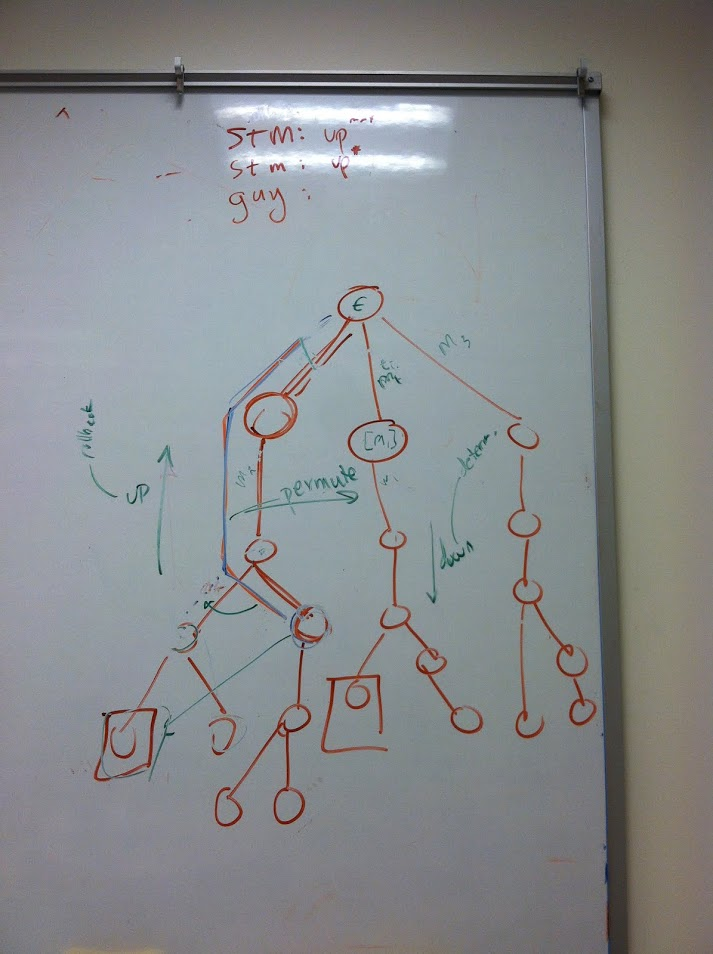
\includegraphics[width=\columnwidth]{tree.jpg}
tree.jpg
\caption{An example}
\label{fig:example}
\end{figure}

We start with a description of all possible interleaved executions of some bounded number of threads, as shown in Figure \ref{fig:example}. Some of the leaf nodes denote admissible final states for the interleaved execution. The rest are inadmissible final states.

A generic concurrent system may produce both admissible and inadmissible executions. Two main approaches have been adopted to produce only admissible executions:
\begin{itemize}
\item apply synchronization to restrict the available parallelism and drive the system only into the admissible executions, and
\item rollback the execution when the system falls into an inadmissible executions, and re-execute the program (sometimes driving the system to avoid to fall back to the inadmissible case already explored).
\end{itemize}

We would like to optimize two properties:
\begin{itemize}
\item Utilization of available parallelism, which is counted as the number of admissible paths that synchronization permits
\item Overhead, which is counted as the number of operation/state reversals that synchronization may force to (re)direct execution toward an admissible final state
\end{itemize}

\todo{for now i guess we just let an operation have unit cost. can
  worry about cost models later}



Our idea is to create a calculus founded on three operations:
\begin{itemize}
\item[Execute] forward execution step
\item[Rollback] local rollback
\item[Permute] a jump to another branch that reflects the same history of operations (but differs in terms of the order of execution of the operations)
\end{itemize}

Once we recognized we fall into an inadmissible execution, our goal is to perform some operations in order to fall into an admissible execution preserving the observable behaviors.
This leads us to two main concepts:
\begin{itemize}
\item What executions are admissible? (in the rest of the paper, we will adopt the classical idea of Software Transaction Memory)
\item What behaviors of an execution are observable? (in the rest of the paper, we will consider final states as the observable behaviors of an execution)
\end{itemize}

We can plug in our approach different definitions of admissible executions, and observable behaviors.

In addition, we want to formalize Permute reaching a node in the tree that is at the same level of the current one. In this way, we do not rollback the execution, but indeed we advance it by one step as we would do if we were in an admissible execution. Intuitively, this means that our permute can be simulated by $n$ rollbacks followed by $m$ execution steps, with $m==n$\footnote{We discussed also the case in which $m>n$, but we are not yet sure if this case will be never interesting}.

\begin{figure}
\begin{lstlisting}
T1:
	put(k,v)
	get(k)

T2:
	remove(k)
\end{lstlisting}
\caption{The running example}
\label{lst:runningexample}
\end{figure}

\begin{figure}[ht]
%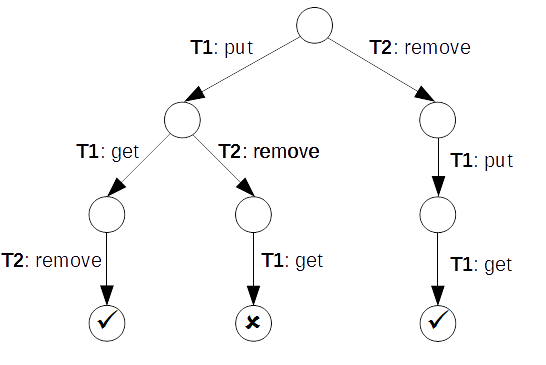
\includegraphics[width=\columnwidth]{treerunningexample.png}
treerunningexample.png
\caption{The tree of executions of the running example}
\label{fig:treerunningexample}
\end{figure}

Consider for instance the running example in Figure \ref{lst:runningexample}.
Figure \ref{fig:treerunningexample} depicts the tree of all possible executions of the running example. We consider the first and last execution as admissible, while the second one is not. This is a quite standard assumption for our running example: The two instructions of T1 conflict with the instruction of T2 (they all work on the same collection and on the same key). Therefore, the system should not allow T2 to execute its instruction if T1 has execute the first instruction but not the second one yet. This is usually achieved in two ways:
\begin{itemize}
\item by synchronization mechanisms (e.g., locks) providing mutual exclusion between T1 and T2, or
\item by rolling back the execution if the system falls into the second path and when executing remove.
\end{itemize}

Instead, we propose a novel approach.
Consider the second path, and the situation in which we have already exposed history \statement{[T1: put, T2: remove]}.
If we refrain from executing remove (that is, we replace it with a skip statement), we would apply a Permute step, that would yield us to the history	\statement{[T2: remove, T1: put]}

In this way, the entire execution becomes \statement{[T2: remove, T1: put, T1: get]} that is an admissible execution.

Note that in contrast with Rollback and Execute, Permute requires an algebraic specification that permits efficient (bounded) editing of the state reflected by \statement{[T1: put, T2: remove]} to arrive at \statement{[T2: remove, T1: put]}.




\section{Permuting the execution -- previous}
The goal of our work is to try to \emph{redirect} a bad execution into a good one by simulating the good trace up to that point. At a given point of an execution, we suppose that we can observe only two things:
\begin{enumerate}
\item where the execution of each transaction is. This can be formalized as $\getTransactionPoints{\tau} = [\statement{t} \mapsto \max(\indexes{\statement{t}}{\tau}) : \statement{t} \in \cset{T}]$
where $\cset{T}$ contains all the identifiers of the transactions in the execution $\tau$, and $\indexes{\statement{t}}{\tau}=\{\cel{i} : \exists \cel{\sigma}_j \to_{(\statement{t}, \cel{i})} \cel{\sigma}_{j+1} \in \tau\}$
\item what we can observe on the last state of the trace. The observational portion of the state is given by a function $\observe{\sigma}$.
\end{enumerate}

Given a bad trace $\sigma_0 \to \cdots \to \sigma_i$ we want to find a good trace $\sigma'_0 \to \cdots \to \sigma'_j$ such that
\begin{enumerate}
\item $\getTransactionPoints{\sigma_0 \to \cdots \to \sigma_i} = \getTransactionPoints{\sigma'_0 \to \cdots \to \sigma'_j}$
\item $\observe{\sigma_0}=\observe{\sigma'_0}$
\item $\observe{\sigma'_j} = \observe{f(\sigma_i)}$ where $f$ is a function that \emph{adjusts} the state of the bad execution to fall into the good execution.
\end{enumerate} 

The two parameters of our framework are $f$ (and a key component is how to compute it) and $\observe{\sigma}$. We suppose that $\observe{\sigma}$ returns the portion of the state that influences what is observable "through" the semantics. This means that if we take two states equivalent modulo observability and we perform the semantics of a statement, we obtain two states that are equivalent modulo observability. Formally,
\[
\begin{array}{c}
\forall \sigma, \sigma' \in \cstates : \observe{\sigma}=\observe{\sigma'} , \forall \statement{s} \in \statements : \langle \statement{s}, \sigma \rangle \to \sigma_1, \langle \statement{s}, \sigma' \rangle \to \sigma'_1\\
\Downarrow\\
\observe{\sigma_1}=\observe{\sigma'_1}\\
\end{array}
\]

Based on the permutation function $f$ we define the semantics $\csemantics{S_{P}}{\statement{p}, \sigma_0}$ that, if the execution falls into a bad trace, redirects the execution into a good trace by applying $f$.\todo{Formalize it, not clear when exactly we apply the permutation}

We can now prove the soundness of our permutation. Intuitively, we prove that if one can observe only the observable part of the entry and the exit state (and not the intermediate state and the interleaving of transactions) it cannot notice the permutation we operate.

\begin{theorem}[Soundness of the permutation]
\[
\forall \sigma_0 \to \cdots \to \sigma_i \in \csemantics{S_{P}}{\statement{p}, \sigma_0}, \exists \sigma_0 \to \cdots \to \sigma'_j \in \csemantics{S}{\statement{p}, \sigma_0} : \observe{\sigma_i} = \observe{\sigma_j}
\]
\todo{Should we relax on the entry state using observe?}
\end{theorem}






\section{New ideas of the meeting on May, 2nd}

\subsection{Observational Equivalence}
Instead of using the idea of an $\mathit{observe}$ function and ask that the states are equal, we can rely on the observational equivalence relation between states. Another approach could be to adopt the POPL 02 Cousot and Cousot framework to define program transformations. First Pietro's intuition: "They deal with online and offline program transformation, and they define observational equivalence as an equivalence among abstractions of concrete executions. Indeed, what we are doing is slightly different: we perform a static analysis offline, and we change the semantics of the program (that - maybe - can be interpreted as a program transformation) online if we fall into a bad execution. On the other hand, I think that we could plug our work into their framework, and the main advantage would be to define the observational equivalence as an abstraction, and in particular as the abstraction we are performing in TVLA. In this way, we won't need to develop an ad-hoc definition of the correspondence between the observational equivalence and what we track with our static analysis."

\subsection{Product of CFGs}
We came up to the idea that in order to represent the interleaving of various threads. If we have two threads T1 and T2, we build up the product of all the nodes, and we add the edges that performs a step in the execution of one of the two threads. In this way we have some spurious paths (e.g., if we are inside a thread performing a loop and we perform one step in the other thread, also this step will be inside the loop), that we should refine through the abstract domain (e.g., adding program pointers of the various threads in the abstract state). In addition, we may have that a bad and a good trace are later joined. In order to distinguish between good and bad traces we will need to partition these two cases in the abstract domain (e.g., through a Bad abstraction predicate in TVLA).

Another idea from Eric was to use his PLDI 09 work (where they perform a sort of loop unrolling by expanding the CFG) but we didn't discuss it in the details.



\end{document}

%%% Local Variables: 
%%% mode: latex
%%% TeX-master: t
%%% End: 
